We consider the discrimination of two electromagnetic signals with opposite phases, described by two coherent states of the field, $\ket{\pm\alpha}$, whose energy is proportional to $|\alpha|^{2}$. When the energy of the signals approaches zero, i.e., $|\alpha|^{2}\ll1$, quantum effects become evident and it becomes impossible to discriminate between them perfectly.

Let us begin by considering measurements that can be carried out in order to infer the value of a bit $k\in\llaves{0,1}$, which is encoded in the phase of a coherent state $\ket{\alpha_k}$, with $\alpha^{(k)} = (-1)^{k}\alpha$. The Wigner function of the two candidate states is shown in Fig~\ref{fig:wigner_312_coh_noiseless}, where the non-vanishing overlap can be appreciated.

\begin{figure}[t]
    \centering
    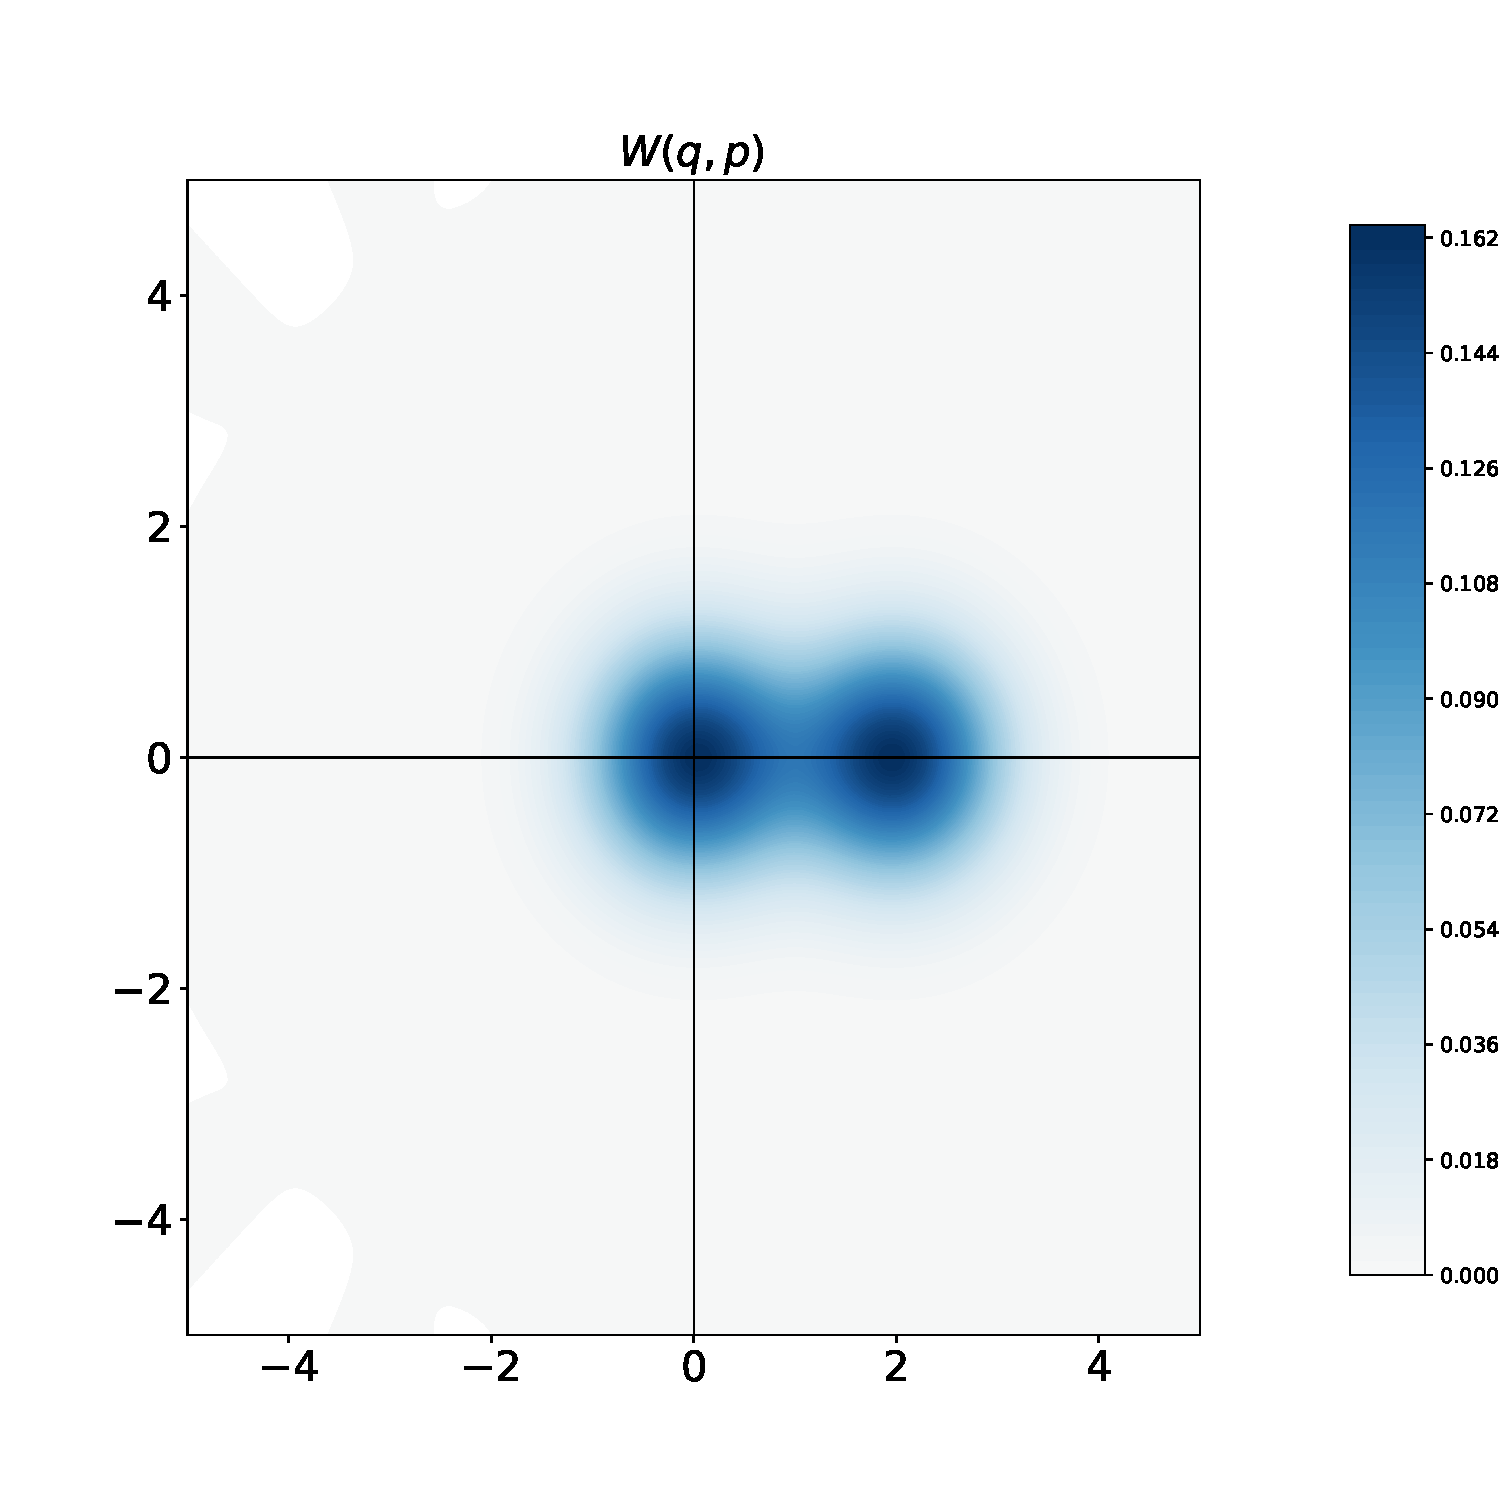
\includegraphics[width=0.5\textwidth]{Figures/312/wigner_coh_displaced.pdf}
    \caption{We show the Wigner function for the state $\rho = \frac{1}{2}\big(\proj{\alpha_0} + \proj{\alpha_1}\big)$, which corresponds to the probabilistic preparation of either $\alpha_0$ or $\alpha_1$ (with equal priors). While the centers of the distribution are distinguishable at first glance, we notice some overlap between the Gaussian distributions appears. Such an overlap behaves like $|\braket{\alpha}{-\alpha}|^2 \propto e^{-|\alpha|^2}$, and thus increases when the intensity of the incoming signal decreases.}
    \label{fig:wigner_312_coh_noiseless}
\end{figure}

As discussed in Sec.~\ref{ssec:1_qdisc}, any binary discrimination protocol is described compactly by a POVM, $\mathcal{M}=\llaves{M_{0},M_{1}}$ with $M_{1,2}\geq0$ and $M_{1}+M_{2}=\mathbb{I}$. The probability of obtaining measurement outcome $\hat{k}$ given that hypothesis $k$ was true is given by $p(\hat{k}|\alpha_k) = \tr{M_k \proj{\alpha^{(k)}}}$.
Nevertheless, once outcome $\hat{k}$ has been obtained, \textit{a guess} for $k$ needs to be done, and the best one is --- by definition ---  related to the most likely hypothesis $k\in\llaves{0,1}$, given outcome $\hat{k}$. Thus, the success probability of this setting reads
\begin{align}
P_{s}(\alpha,\mathcal{M})&=\sum_{\hat{k}=0,1}\max_{k=0,1}p(\alpha^{(k)},\hat{k})\\
&=\sum_{\hat{k}=0,1}\max_{k=0,1}p(\hat{k}|\alpha^{(k)})p_{k}.
\end{align}
